\documentclass{article}
\usepackage{listings}             % Include the listings-package
\usepackage[usenames,dvipsnames,svgnames,table]{xcolor}
\usepackage{graphicx}
\usepackage{hyperref}
\usepackage{amsmath}
\usepackage{csquotes}
\usepackage{changelog}

\definecolor{mygreen}{rgb}{0,0.6,0}
\definecolor{mygray}{rgb}{0.5,0.5,0.5}
\definecolor{mymauve}{rgb}{0.58,0,0.82}

\newcommand{\ChatDiamondVersion}{0.1.0-alpha}
    
\title{Chat Diamond}
\author{The\_Cowboy}
\pagestyle{headings}
\begin{document}
\maketitle
\lstset{language=Java}          % Set your language (you can change the language for each code-block optionally)
\section{Introduction}

\lstset{ %
  backgroundcolor=\color{white},   % choose the background color; you must add \usepackage{color} or    %\usepackage{xcolor}
  basicstyle=\footnotesize,        % the size of the fonts that are used for the code
  breakatwhitespace=false,         % sets if automatic breaks should only happen at whitespace
  breaklines=true,                 % sets automatic line breaking
  captionpos=b,                    % sets the caption-position to bottom
  commentstyle=\color{mygreen},    % comment style
  deletekeywords={...},            % if you want to delete keywords from the given language
  escapeinside={\%*}{*)},          % if you want to add LaTeX within your code
  extendedchars=true,              % lets you use non-ASCII characters; for 8-bits encodings only, %does not work with UTF-8
  frame=single,                    % adds a frame around the code
  keepspaces=true,                 % keeps spaces in text, useful for keeping indentation of code %(possibly needs columns=flexible)
  keywordstyle=\color{blue},       % keyword style
  language=Java,                 % the language of the code
  morekeywords={*,...},            % if you want to add more keywords to the set
  numbers=left,                    % where to put the line-numbers; possible values are (none, left, %right)
  numbersep=5pt,                   % how far the line-numbers are from the code
  numberstyle=\tiny\color{mygray}, % the style that is used for the line-numbers
  rulecolor=\color{black},         % if not set, the frame-color may be changed on line-breaks within %not-black text (e.g. comments (green here))
  showspaces=false,                % show spaces everywhere adding particular underscores; it %overrides 'showstringspaces'
  showstringspaces=false,          % underline spaces within strings only
  showtabs=false,                  % show tabs within strings adding particular underscores
  stepnumber=2,                    % the step between two line-numbers. If it's 1, each line will be %numbered
  stringstyle=\color{mymauve},     % string literal style
  tabsize=2,                       % sets default tabsize to 2 spaces
  title=\lstname                   % show the filename of files included with \lstinputlisting; also %try caption instead of title
} %optionally)

ChatDiamond is a purely client-side mod for Unreal Tournament G.O.T.Y which relplaces the default UT console with a more appropriate one.  This functionality allows the achievement of the following
\begin{itemize}
\item Gathering of raw messages delivered to the console and relevant categorization, along with chat message seperation, of them.
\item Introduction of appropriate web-query for translation to local or demand of the language.
\end{itemize}

\begin{figure}
\centering
\label{fig:chatdiamond}
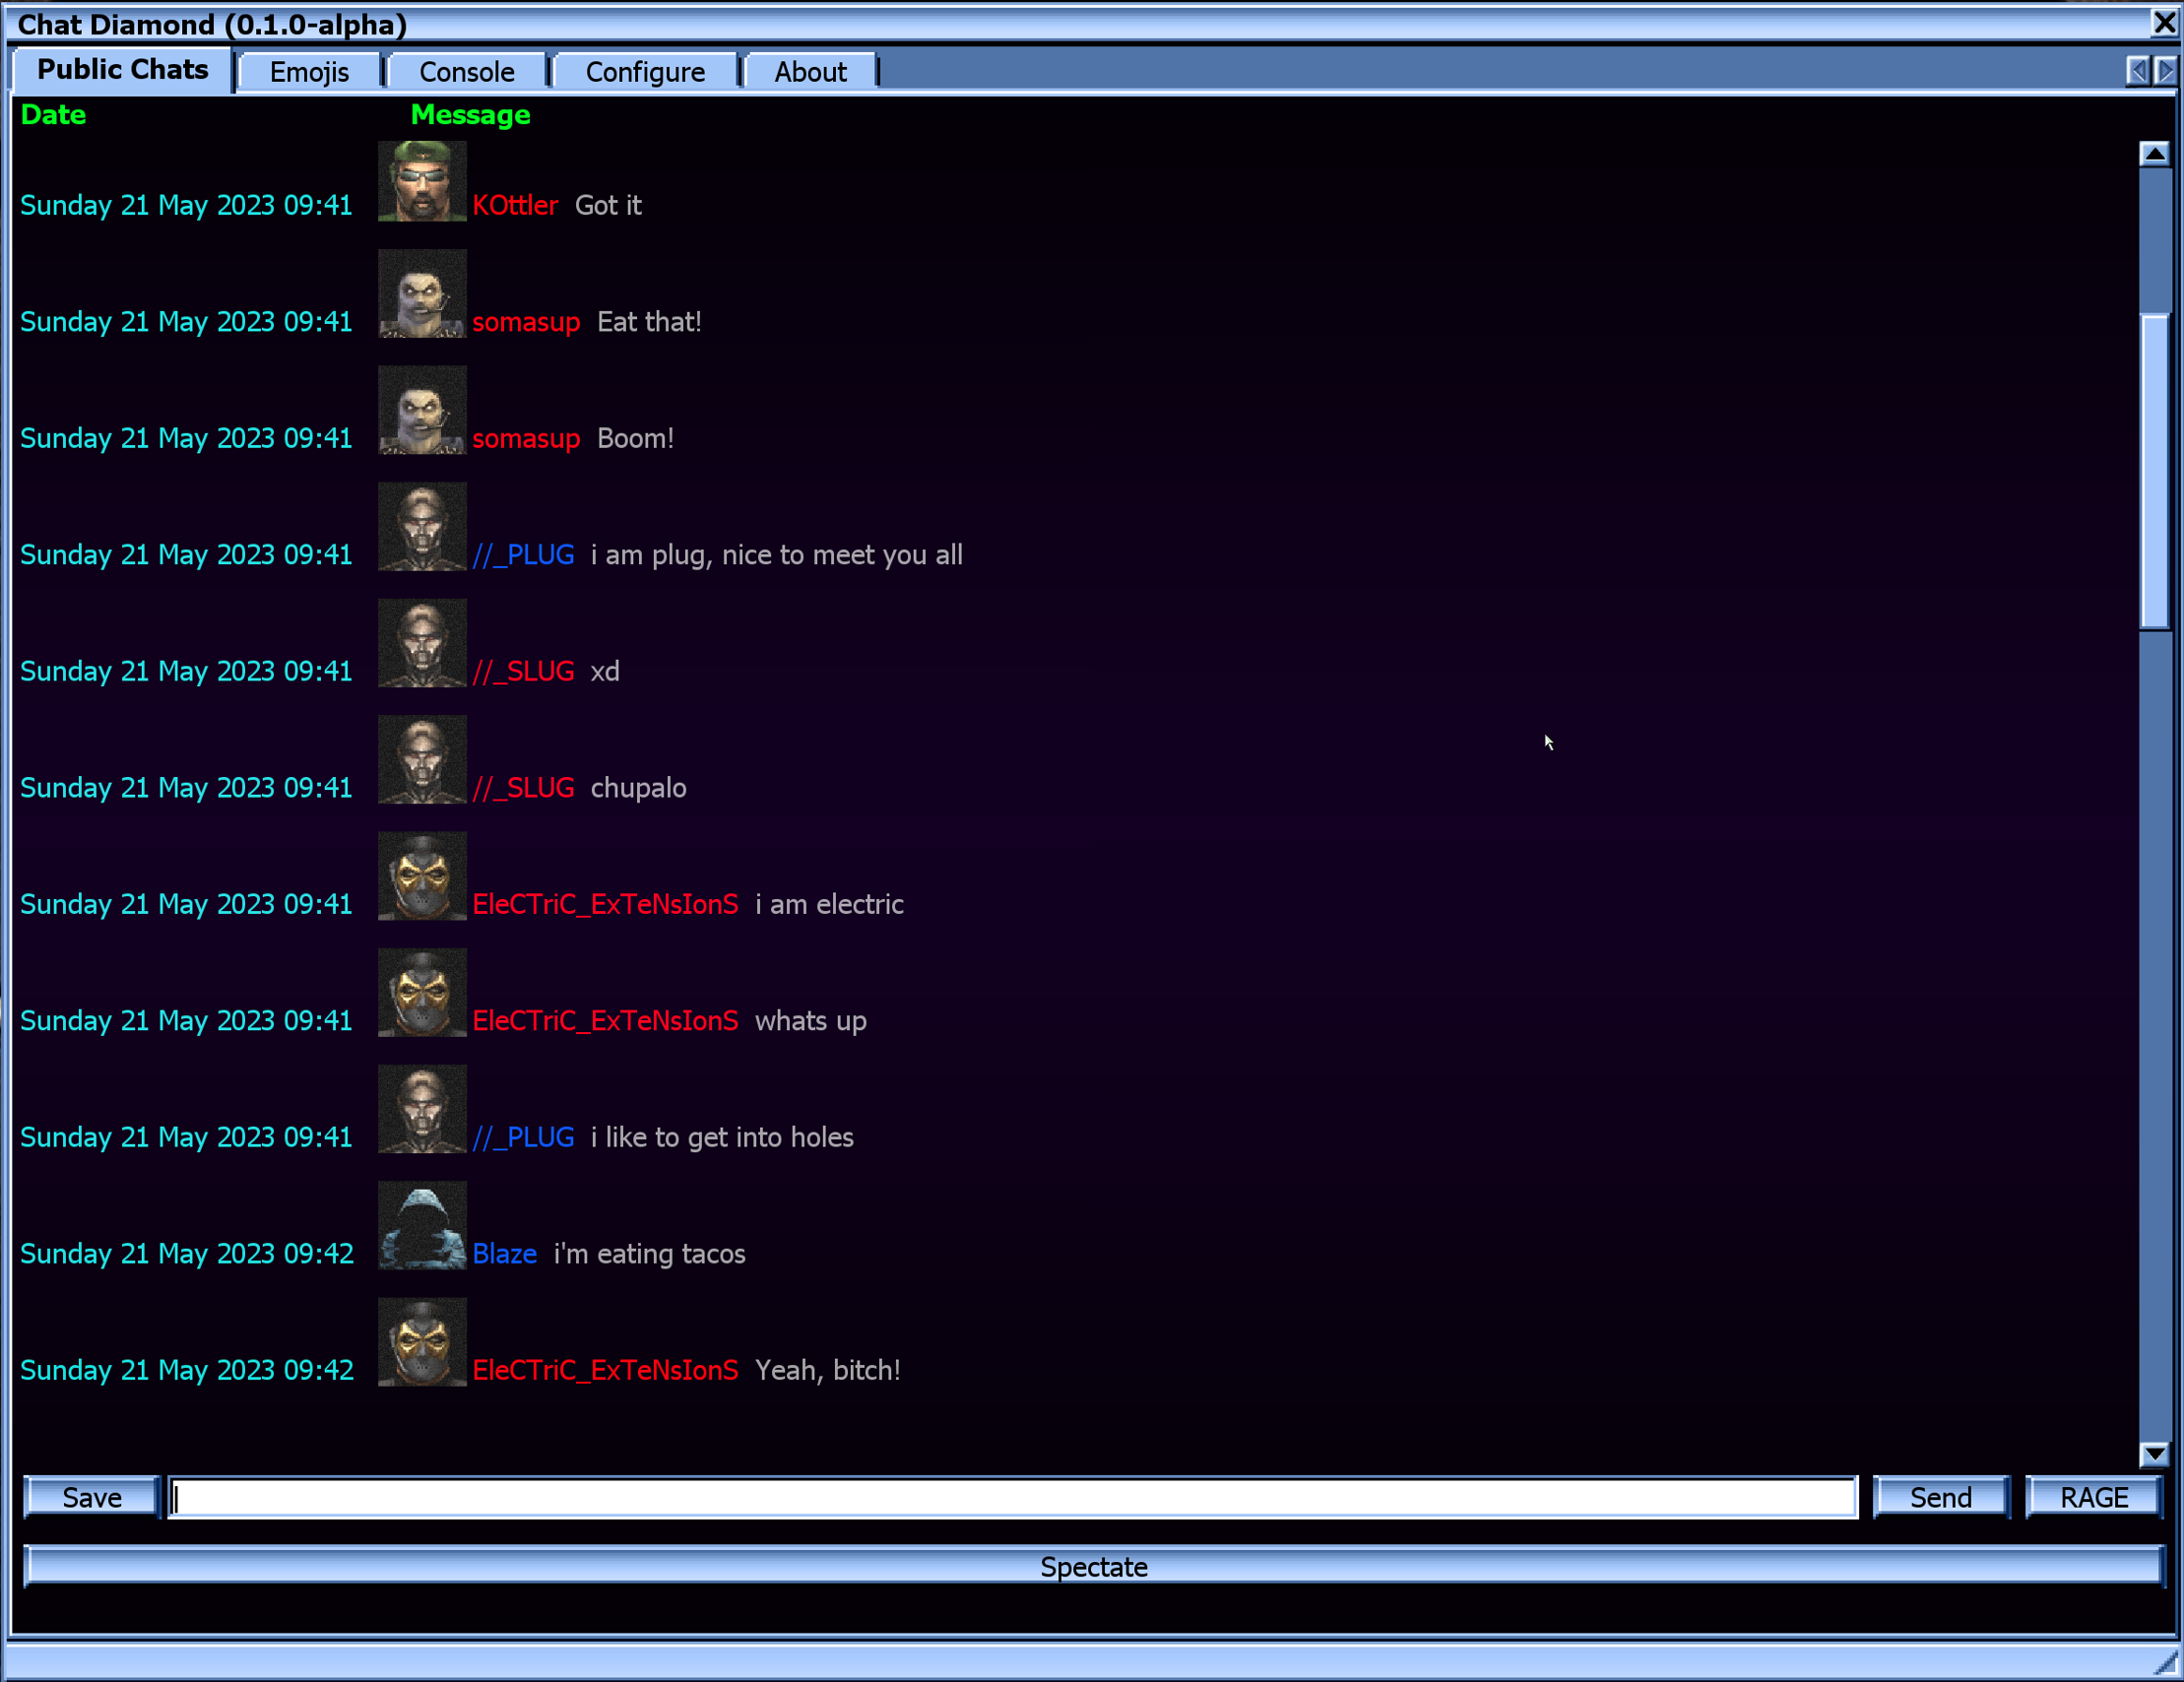
\includegraphics[width=0.4\textwidth]{img}
\caption{A screenshot of the ChatDiamond \ChatDiamondVersion~chat}
\end{figure}

\subsection{Chat Window}
Figure \ref{fig:chatdiamond} shows the current form of the chat window. The following features are supported
\begin{itemize}
\item Display of sender's avatar face.
\item Static emojis and animated emotes.
\item Display of Date and Time (long format for now).
\item Display of the Server name for reference purposes.
\end{itemize}

\subsection{Console Window}
\begin{figure}
\centering
\label{fig:chatdiamond_console}
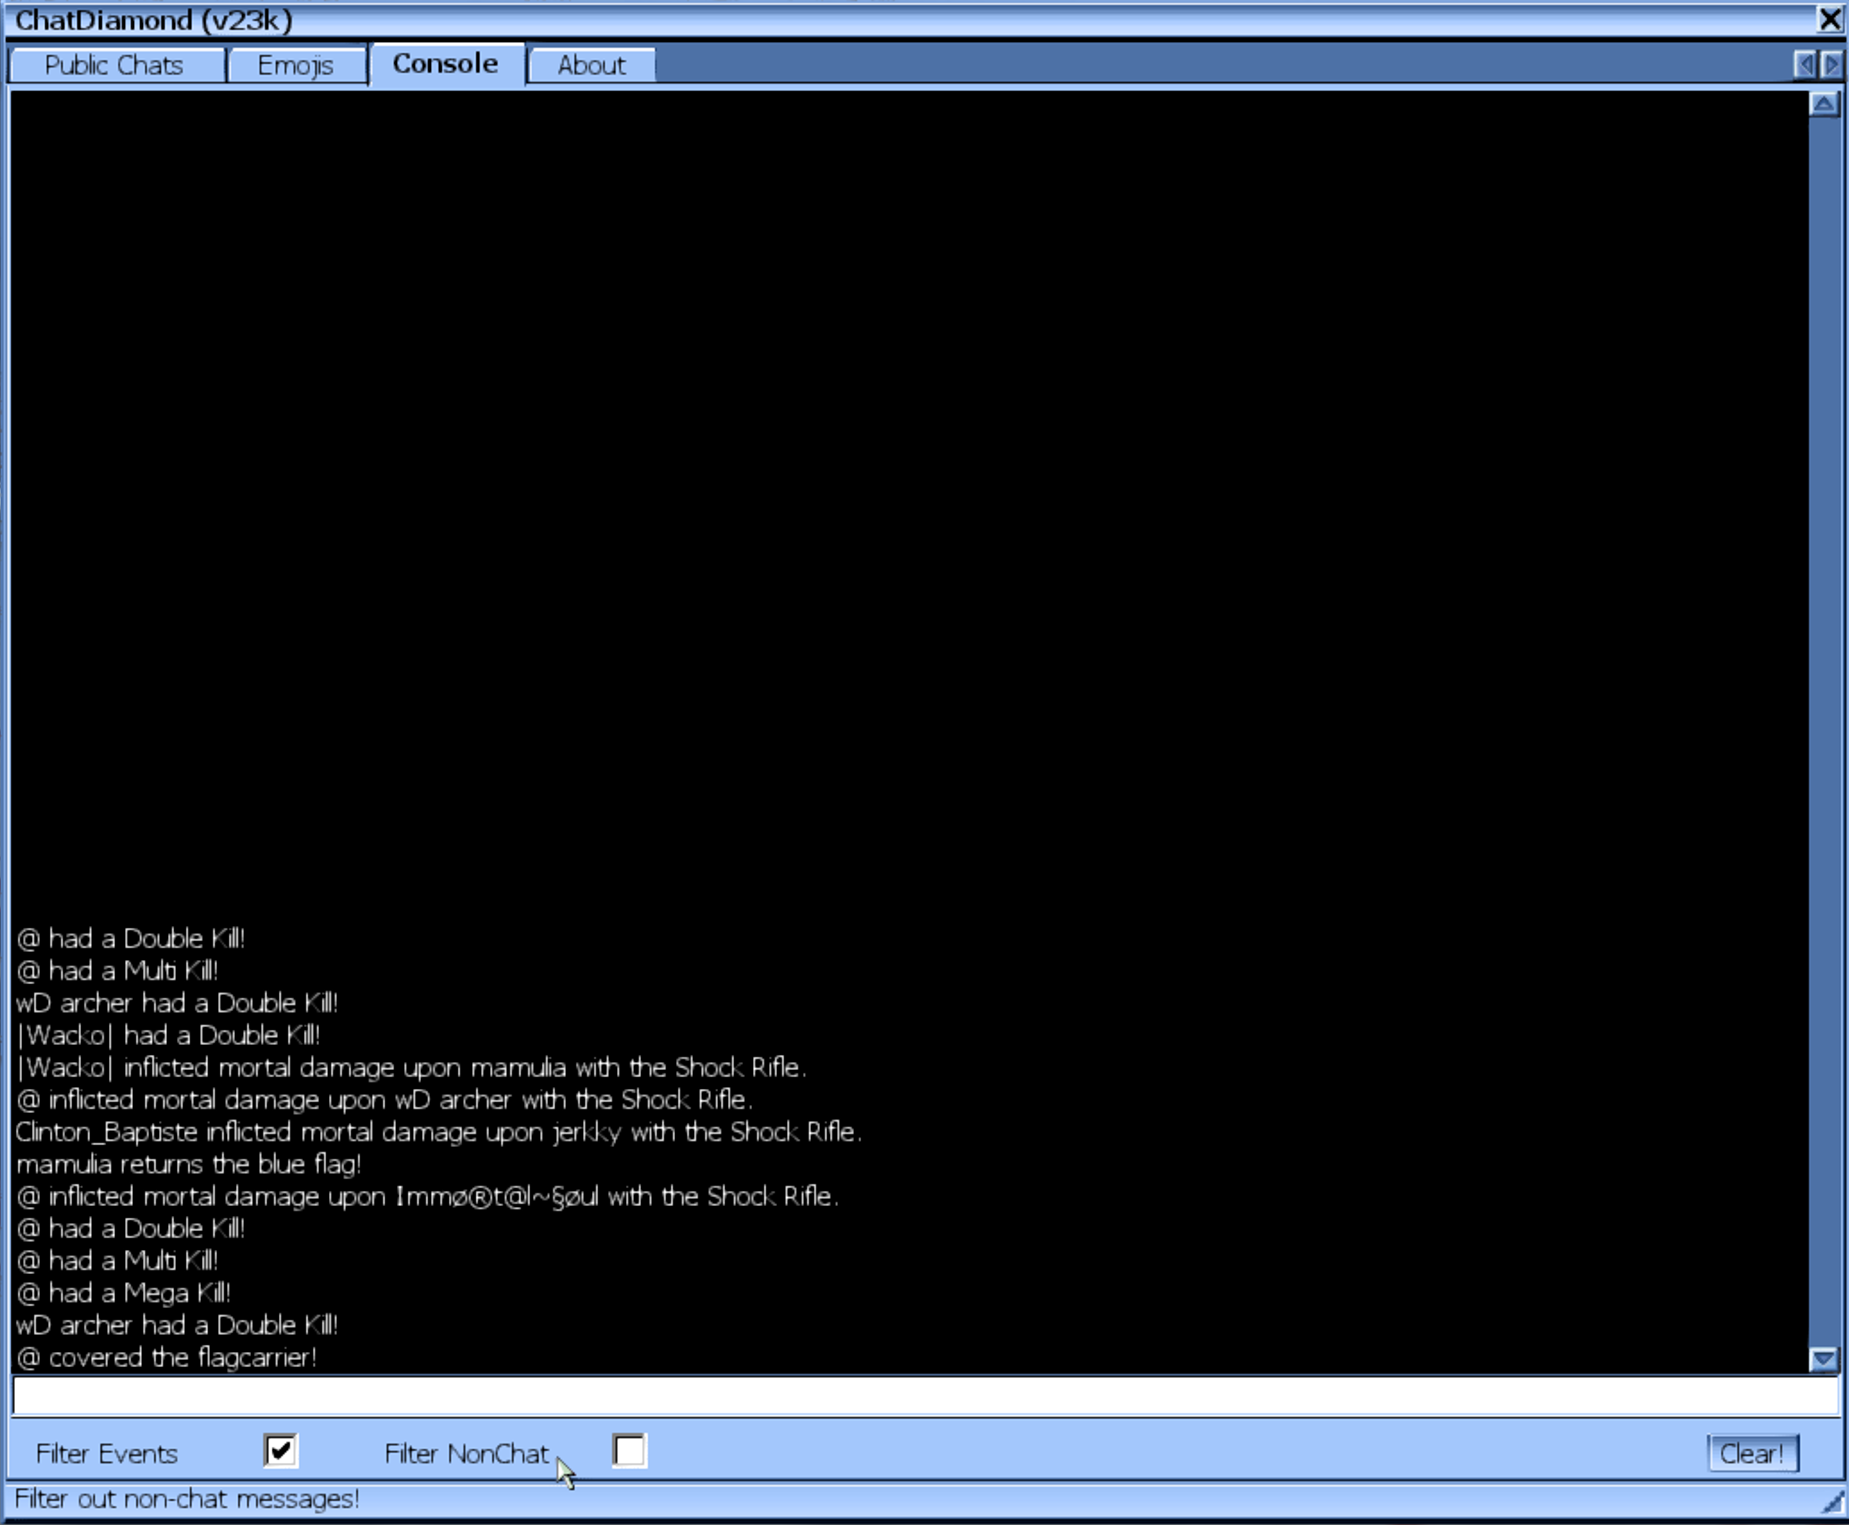
\includegraphics[width=0.4\textwidth]{img_console}
\caption{ChatDiamond \ChatDiamondVersion~console}
\end{figure}

The console now has the following features
\begin{itemize}
\item Non-chat filter to filter out server or mutator advertisements, in the console. Although SmartCTF cover and seal messages may also get filtered.
\item Event filter censors death messages corresponding to the weapon used.
\item A clear button to clean or reset the console.
\item A working status bar linked with console configuration modifiers.
\end{itemize}



\end{document}